%!Tex Root = ../Tutorat4.tex
% ./Packete.tex
% ./Design.tex
% ./Deklarationen.tex
% ./Aufgabe1.tex
% ./Aufgabe2.tex
% ./Bonus.tex

\section{Task 3}

\setcounter{task}{1}

\begin{frame}{Task 3}{Scheduling with Polling Server}
  \begin{tasknoinc}
    \begin{figure}
       \centering
       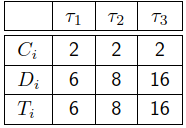
\includegraphics[scale=0.8]{figures/periodic_tasks_3.1.PNG}
       \label{fig:my_label}
   \end{figure}
   \begin{itemize}
       \item In addition to the above periodic tasks, we have an aperiodic job $J_a$ with $C_a = 1$ and relative deadline $D_a$. Let $T_s = 25$ and $C_s = 1$ respectively, where $T_s$ denotes the period and $C_s$ the computing time (or capacity) of the polling server (PS)
       \item Compute the minimum relative deadline of $J_a$ which is guaranteed not to be missed, that is, its aperiodic guarantee.
   \end{itemize}
  \end{tasknoinc}
\end{frame}
\begin{frame}[allowframebreaks]{Task 3}{Scheduling with Polling Server}
    \begin{solutionnoinc}
      \begin{itemize}
          \item As reminder: The polling server itself acts like a \alert{periodic} task, that uses its capacity to serve \alert{aperiodic} tasks. If the polling server has the current highest priority it begins to serve any pending aperiodic requests within the limits of its capacity.
          \item If there are no pending aperioidic tasks at that time it \alert{suspends} its entire capacity! (until the beginning of the next period)
          \item Therefore, the worst possible case occurs when $J_a$ appears slightly later than the polling server checks for pending aperiodic tasks. Meaning, the polling server suspends its capacity and $J_a$ has to wait $T_s + \lceil \frac{C_a}{T_s}\rceil T_s = (1 + \lceil \frac{C_a}{T_s}\rceil)T_s$
      \end{itemize}
    \end{solutionnoinc}
    \framebreak
    \begin{solution}
      \begin{itemize}
          \item To guarantee to not miss the deadline $D_a$ the condition $(1 + \lceil \frac{C_a}{T_s}\rceil)T_s \leq D_a$ needs to hold.
          \item Entering the values for the exercise gives us $D_a = 50$
      \end{itemize}
    \end{solution}
    \begin{Sidenote}
      Note that the above computation of course only holds if the RM schedule meets all the deadlines.
    \end{Sidenote}
\end{frame}
\begin{frame}{Task 3}{Scheduling with Polling Server}
    \begin{tasknoinc}
    Using the sufficient test of RM, test if the polling server of task 3.1 is schedulable along with the periodic task-set.
    \end{tasknoinc}
\end{frame}
\begin{frame}{Task 3}{Scheduling with Polling Server}
    \begin{solutionnoinc}
    \begin{itemize}
        \item We have already seen the sufficient but not necessary condition of $\sum\limits_{i=1}^{n}\cfrac{C_i}{T_i} \leq n(2^{1/n}-1)$ for rate monotonic scheduling.
        \item The convenient part about our polling server: we can just treat it as an additional \alert{periodic} task.
        \item Therefore, the same test offers us a sufficient condition for rate monotonic scheduling with a polling server! Simply increase from n tasks to (n+1)
        \item Check: $\sum\limits_{i=1}^{n}\cfrac{C_i}{T_i} \quad + \underbrace{\frac{C_s}{T_s}}_{\text{server task}} \leq (n+1)(2^{1/(n+1)}-1)$
    \end{itemize}
    \end{solutionnoinc}
\end{frame}
\begin{frame}{Task 3}{Scheduling with Polling Server}
    \begin{solution}
    \begin{itemize}
        \item Putting in values we obtain: $0.748 \leq 0.76$. Since this is true, we know (as this is a sufficient condition) that the RM schedule meets all deadlines!
    \end{itemize}
    \end{solution}
\end{frame}
